%----------------------------------------------------------------------------------------
%	PACKAGES AND DOCUMENT CONFIGURATIONS
%----------------------------------------------------------------------------------------

\documentclass{article}

\usepackage{graphicx} % Required for the inclusion of images

\usepackage[utf8]{inputenc}

\usepackage[justification=centering]{caption}
\usepackage{caption}
\usepackage{subcaption}
\usepackage{amsmath,amssymb,amsfonts,amsthm,mathtools}
\usepackage{xfrac}
\usepackage{float}

\usepackage{hyperref}
\usepackage{url}
\usepackage{array}
\usepackage[flushleft]{threeparttable}

\usepackage{comment}
\usepackage[font=small,labelfont=bf]{caption}


\usepackage{listings, lstautogobble}
\usepackage{fancyhdr}
\usepackage{graphicx}
\usepackage{hyperref}

\graphicspath{ {./} }
\setlength\parskip{4pt}
\setlength\parindent{0pt}
\setlength{\tabcolsep}{8pt}
\renewcommand{\arraystretch}{1.5}
% \setlength{\tabcolsep}{8pt}
% \renewcommand{\arraystretch}{1.5}

%\usepackage{times} % Uncomment to use the Times New Roman font

%----------------------------------------------------------------------------------------
%	DOCUMENT INFORMATION
%----------------------------------------------------------------------------------------

\title
{
	\LARGE\textbf{Dog detection} \\ 
	Neural network course project \\
	\author
	{ 
		Jakub \textsc{Zadrożny}, 
		Mateusz \textsc{Hazy},
		Kamil \textsc{Szubiński}
	}
}
\date{\today}

\begin{document}
\maketitle

\section*{Abstract}

Object detection is a very rapidly evolving deep learning area and a wide variety of methods has been developed in recent years. Many of them suffer from a computation complexity (RCNN). In this paper we revisit YOLO \cite{yolo} and YOLO v2 (introduced in YOLO9000 paper \cite{yolo9000}) - fast real time object detection methods. Both of them are able to detect many classes of objects, however, we limit ourselves to detecting only one class - a dog. We then compare both versions of YOLO to seek for any improvement.

\section*{YOLO}

The YOLO method states detection as a linear regression problem straight from pixels to bounding boxes coordinates and class probabilities. The system divides image into $ S \times S $ grid. If the center of an object falls into a grid cell, that grid cell is responsible for detecting that object. Each grid cell can predict $B$ bounding boxes. Each bounding box consists of five predictions: $x, y, w, h$ and confidence, where the first four describe the bounding box location and size. The last parameter describes how confident the model is that the bounding box contains the object. Overall the YOLO architecture takes the image, passes it through convolutional and fully connected layers and produces $S \times S \times (B \cdot  5 + C)$ predictions. Each $B \cdot 5 + C$ segment represents the predictions for the grid cell. Five parameters described above for each bounding box and C class probabilities. The original paper \cite{yolo} provides more detailed description.

\section*{YOLO v2}

The YOLO v2 is in fact the basic YOLO with several improvements. For example, the use of batch normalization on all convolutional layers in YOLO not only eliminates the need for other forms of regularisation (in theory), but also results in $2\%$ improvement in mAP. Further changes include higher resolution classifier (denser grid) and direct location prediction. \\
The last improvement is very useful for dealing with initial instability. In region proposal networks the network predicts values $t_x$ and $t_y$ and the $(x,y)$ center coordinates are calculated as
\begin{equation}
\begin{aligned}
x &:= (t_x \cdot w_a)-x_a \\
y &:= (t_y \cdot h_a)-y_a
\end{aligned}
\end{equation}
Since this formulation is unconstrained, any anchor box can end up at any point in the image. To overcome this drawback, we bound the location using logistic activation $\sigma$, which makes the value fall between $0$ to $1$:
\begin{equation}
\begin{aligned}
b_x &:= \sigma(t_x) + c_x \\
b_y &:= \sigma(t_y) + c_y \\
b_w &:= p_w \cdot e^{t_w} \\
b_h &:= p_h \cdot e^{t_h} \\
\end{aligned}
\end{equation}
according to \textbf{Figure 1}.\\
\begin{figure}
\centering
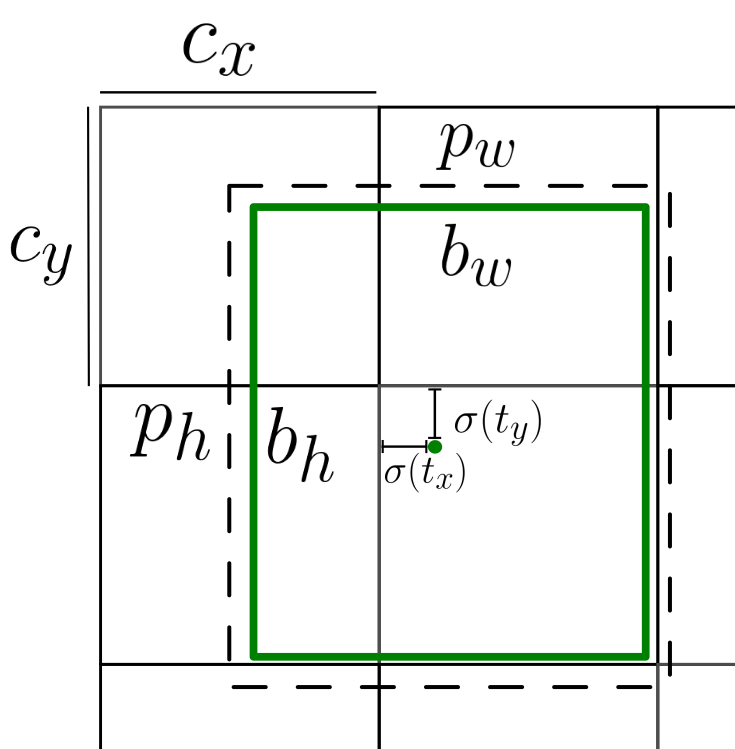
\includegraphics[scale=0.25]{scheme.png}
\caption{Direct location prediction.}
\end{figure}
This technique results in $5\%$ increase in mAP over the version of anchor boxes.
\\ More detailed description is available in the paper.

\section*{Dataset}
We decided to use a subset of Youtube-BoundingBoxes Dataset \cite{youtube-bb}. One can find there more than 200000 frames with dogs. The biggest disadvantage of this dataset is that only one object is detected in every frame. This can lead to some troubles with learning the model. The other problem is that some bounding boxes are set incorrectly. However, this can reduce overfitting during learning.
Furthermore, we employed data augumentation, namely random translations (up to 25 px) and random rotations (up to 25 degrees).

\begin{figure}[H]

\begin{minipage}{.4\textwidth}
	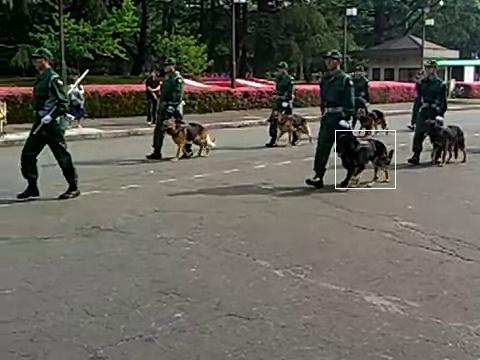
\includegraphics[width=\textwidth]{multiple_dogs.jpg}
	\caption{Image with many dogs, where only one is detected.}
\end{minipage}%
\hfill
\begin{minipage}{.4\textwidth}
	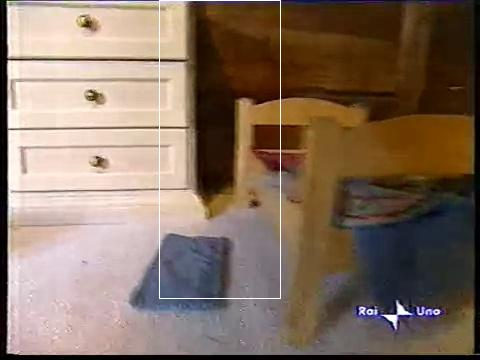
\includegraphics[width=\textwidth]{wrong_bb.jpg}
	\caption{Image with wrong bounding box.}
\end{minipage}%
\hfill

\end{figure}


\section*{Training}

We took 8000 of the images of dogs from Youtube-BoundingBoxes Dataset and did traditional train/test split. Then we used Adam as an optimizer. \\

We optimized the weighted mean least squares error, as suggested in the paper \cite{yolo} \\

The error function was defined as:
$$ 1 - IOU(predicted\_box, true\_box)$$
where
$$ IOU(A, B) = \frac{ A \cap B}{A \cup B} $$

\subsection*{YOLO training}
As a feature extractor we tried to use pretrained vgg and resnet50 networks (documented in \cite{models}). On top of that we added 2 fully connected layers and ReLU for nonlinearity. For regularization we used dropout with $p = 0.5$. 

\begin{figure}[H]
	\begin{center}
		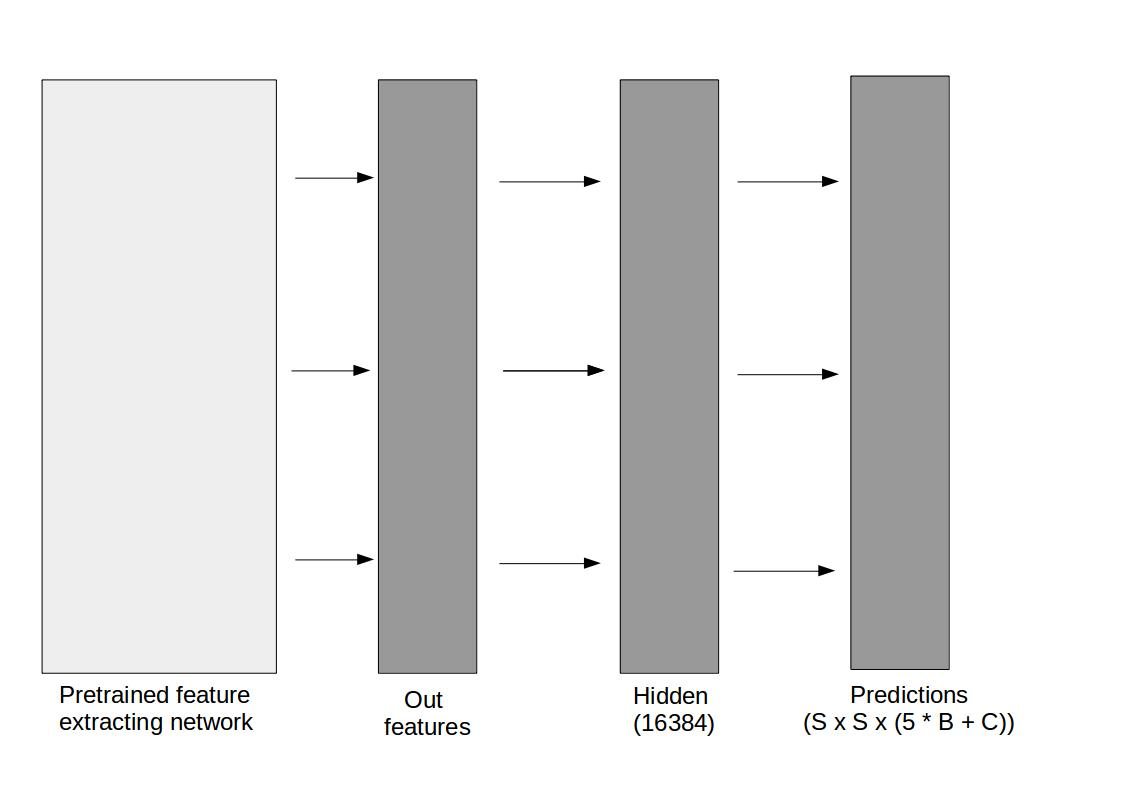
\includegraphics[width=10cm]{yolo_arch.jpg}\\
		\centering
		\caption{YOLO architecture}
	\end{center}
\hfill

\end{figure}

We managed to train the network down to 25\% train error rate. However the test error rate has never been smaller than 65\%. We tried different configurations of hyperparameters, adding noise to input values and data augmentation, yet it did not improve the results. We decided to abandon the YOLO approach and move to the YOLO 9000.

\subsection*{YOLO 2 training}

To get good anchor boxes, we ran K-means on bounding boxes from the dataset. However the closest centroid was chosen not by euclidean distance but by the best IOU score. 

As a feature extractor we used again resnet50, but instead of fully connected layers, we added 4 convolutional layers on top of it. Each convolutional layer was followed by batch normalisation and ReLU.

As a result we managed to reduce test error rate down to 48\% which we found satisfying.


\section*{Conclusion}

Although we did not achieve spectacular results, there are some interesting outcomes we noticed.

Our YOLO network had a problem with overfitting. We used dropout and weight decay, but results were not satisfactory enough. YOLOv2 uses batch norm and smaller weight decay, which resulted in much better performance.

Even though we trained the model on the dataset with only on dog per image, it is quite good at finding multiple dogs. If there are two or three dogs on the picture, then top 3 predictions find them. We present two examples below.


\begin{figure}[H]

\begin{minipage}{.4\textwidth}
	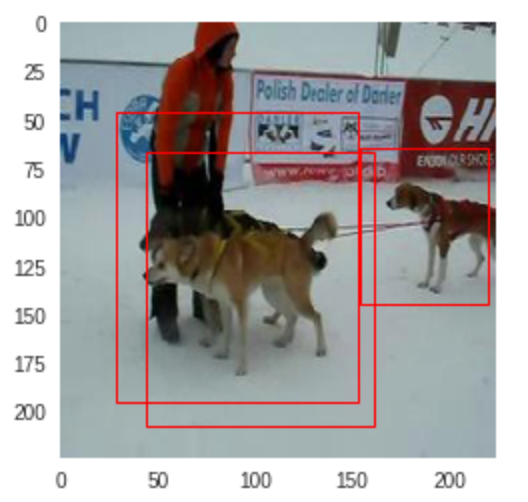
\includegraphics[width=\textwidth]{many_detected1.png}
\end{minipage}%
\hfill
\begin{minipage}{.4\textwidth}
	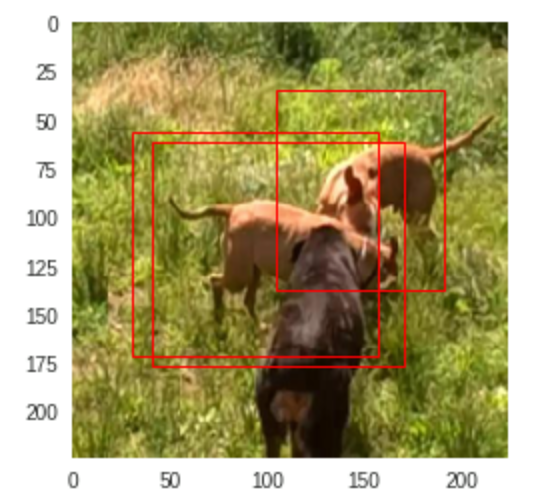
\includegraphics[width=\textwidth]{many_detected2.png}
\end{minipage}%
\hfill

\end{figure}

We consider the failure with YOLO as our mistake. Maybe tuning the model could improve the results. However, it might have been the problem with the dataset quality as well.

Using the anchor boxes int YOLO V2 significantly improves the learning. Intuitively, there are $B$ boxes in each grid cell, because we want to encourage each box to specialize to detect specific type of shape. If the model has good priors of these types, it only has to adjust the boxes, instead of learning from scratch. Moreover, it is worth mentioning that our network can work and learn on images of any size. \\

%\newpage
\begin{thebibliography}{9}

\bibitem{yolo}
Joseph Redmon, Santosh Divvala, Ross Girshick, Ali Farhadi:
\\You Only Look Once: Unified, Real-Time Object Detection
\\\texttt{https://arxiv.org/pdf/1506.02640v5.pdf}

\bibitem{yolo9000}
Joseph Redmon, Ali Farhadi: YOLO9000:Better, Faster, Stronger
\\\texttt{https://arxiv.org/pdf/1612.08242v1.pdf}

\bibitem{youtube-bb}
\texttt{ https://research.google.com/youtube-bb/}

\bibitem{models}
\texttt{ https://pytorch.org/docs/stable/torchvision/models.html }

\end{thebibliography}

\end{document}